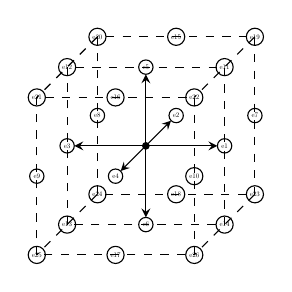
\begin{tikzpicture}
%styledesnœuds
\tikzstyle{textLine}=[rectangle, text=black, scale=0.5]
\tikzstyle{textw}=[rectangle, text=black]
\tikzstyle{pointEi}=[circle, draw, scale=0.25]
%figure
\draw[dashed] (-1,-1,0) rectangle + (2,2,0);
\draw[dashed] (-1,-1,-1) rectangle + (2,2,0);
\draw[dashed] (-1,-1,1) rectangle + (2,2,0);
\draw[dashed] (-1,-1,-1) -- (-1,-1,1);
\draw[dashed] (1,1,-1) -- (1,1,1);
\draw[dashed] (-1,1,-1) -- (-1,1,1);
\draw[dashed] (1,-1,-1) -- (1,-1,1);
%nodes
\node[pointEi, fill] (e0) at (0,0,0) {};

\node[pointEi] (e1) at    (1,0,0) {e1};
\node[pointEi] (e2) at  (0,0,-1) {e2};
\node[pointEi] (e3) at    (-1,0,0)  {e3};
\node[pointEi] (e4) at  (0,0,1)  {e4};
\node[pointEi] (e5) at  (0,1,0) {e5};
\node[pointEi] (e6) at (0,-1,0) {e6};
\node[pointEi] (e7) at    (1,0,-1)  {e7};
\node[pointEi] (e8) at    (-1,0,-1)  {e8};
\node[pointEi] (e9) at    (-1,0,1)  {e9};
\node[pointEi] (e10) at    (1,0,1)  {e10};
\node[pointEi] (e11) at    (1,1,0)  {e11};
\node[pointEi] (e12) at    (-1,1,0)  {e12};
\node[pointEi] (e13) at   (-1,-1,0)  {e13};
\node[pointEi] (e14) at    (1,-1,0)  {e14};
\node[pointEi] (e15) at   (0,1,-1)  {e15};
\node[pointEi] (e16) at   (0,1,1)  {e16};
\node[pointEi] (e17) at   (0,-1,1)  {e17};
\node[pointEi] (e18) at   (0,-1,-1)  {e18};
\node[pointEi] (e19) at    (1,1,-1)  {e19};
\node[pointEi] (e20) at    (-1,1,-1)  {e20};
\node[pointEi] (e21) at    (-1,1,1)  {e21};
\node[pointEi] (e22) at    (1,1,1)  {e22};
\node[pointEi] (e23) at    (1,-1,-1)  {e23};
\node[pointEi] (e24) at    (-1,-1,-1)  {e24};
\node[pointEi] (e25) at    (-1,-1,1)  {e25};
\node[pointEi] (e26) at    (1,-1,1)  {e26};

%text

%vecteur
\tikzstyle{vector}=[-{stealth[scale=0.5]},thin,rounded corners=4pt]
\draw[vector] (e0) -- (e1);
\draw[vector] (e0) -- (e2);
\draw[vector] (e0) -- (e3);
\draw[vector] (e0) -- (e4);
\draw[vector] (e0) -- (e5);
\draw[vector] (e0) -- (e6);
\end{tikzpicture}
